%% Beginning of file 'PASPsample631.tex'

%% using aastex version 6.3.1
\documentclass[twocolumn]{aastex631}
\newcommand{\vdag}{(v)^\dagger}
\newcommand\aastex{AAS\TeX}
\newcommand\latex{La\TeX}


\begin{document}

\title{Properties of Bulge and Disk Particles in the Milky Way and M31 Merger Remnant}

\author{Ellen Jesina}
\affiliation{The University of Arizona\\
Tucson, AZ 85719}

\keywords{Major Merger, Stellar Bulge, Stellar Disk, Local Group, Elliptical Galaxy}

\received{\today}

\section{Introduction} \label{sec:intro}
%Define proposed topic & how it pertains to Galaxy Evolution. Describe the general area of galaxy structure/dynamics and/or evolution

Galaxies have been observed to merge across the Universe, and the closest merger to Earth will involve our very own galaxy and Andromeda, or M31. These galaxies, along with the Triangulum Galaxy (M33), make up the local group that is used to refer to the closest galaxies to Earth and the Milky Way. Eventually, the Milky Way and M31 will collide (\cite{Cox_2008}) which will change the shape and dynamics of the remnant of the merger. In order to better understand how these dynamics have changed, we must observe how the stellar bulge and the stellar disk will change. The stellar bulge is the bright stellar structure that is close to the center of the galaxy, which is commonly surrounding a black hole. The stellar disk involves the stars that are surrounding the center, though at a much farther distance and less concentrated than the stellar bulge, and can often be seen in a spiral pattern for the Milky Way. As the galaxies merge, these components will change in dynamics and relations which can be anticipated by analyzing the merger remnant through coding simulations. 


%State why this topic matters to our understanding of galaxy evolution
This topic is important to understanding how galaxies evolve as they merge overall. The term \textbf{galaxy} is defined as "a gravitationally bound collection of stars whose properties cannot be explained by a combination of baryons and Newton's laws of gravity" (\cite{Willman_2012}).The galaxies undergo evolution through time. \textbf{Galaxy Evolution} is overall dependent on the initial conditions such as temperature and gas mixtures, star formation history, and the gravity interactions between baryonic and dark matter (\cite{Matteucci_2003}). 
By studying galactic evolution, we can determine many interactions, including which particles are more likely to be dynamically changed. Furthermore, studying our own galaxy's evolution can offer us insight into its fate and enable us to better understand its interactions with other galaxies. This can even include how this can impact our own Solar System, since it is likely that this event will occur within the Sun's lifetime (\cite{Cox_2008}). In our case, we are looking into how the remnant of this merger behaves. This remnant, or what is left and formed after the two galaxies merge, is important to understand how different particles behave and evolve so we can understand galactic dynamics more thoroughly. Galaxy mergers are important to study in order to better understand the evolution of galaxies we can observe. The analysis of one or the other can be easily applied to both areas so that we understand galactic dynamics and how the universe has formed as a whole. 

%Overview our current understanding of the topic in galaxy evolution, very broadly
It is commonly understood that the Milky Way and Andromeda will eventually merge due to their gravitational attraction. This is expected to happen in the next 5 Gyr (\cite{Cox_2008}) and can be seen in Figure \ref{Figure 1}. Galaxy mergers are dependent not only on the mass of the galaxies merging (\cite{10.1111/j.1365-2966.2010.16268.x}), but also on the amount of angular momentum (\cite{2008ApJS..175..356H}). It can even depend on the baryonic mass in particular (\cite{10.1111/j.1365-2966.2010.16268.x}), though this is more variable when it comes to smaller galaxy mergers as compared to large galaxies like the Milky Way and Andromeda. Recent research has studied the timescales of this merger (\cite{Cox_2008}), though the explicit dynamics of how our own galaxy will evolve is limited in literature. Much of our understanding comes from how we observe other galaxies merge, visually and dynamically. 

\begin{figure}
    \centering
    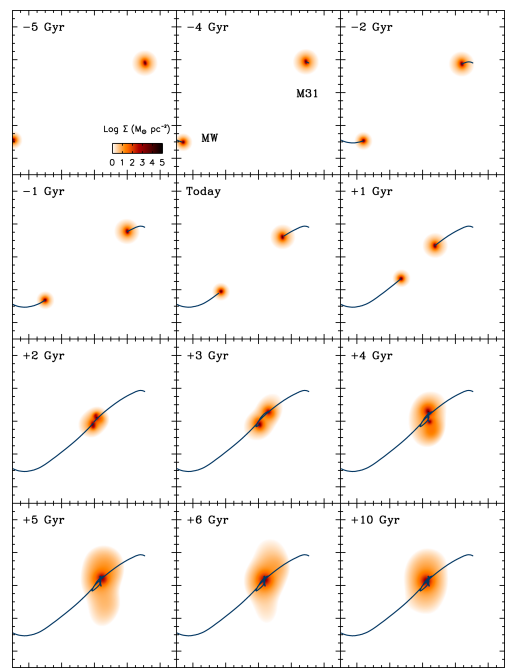
\includegraphics[width = 0.5\textwidth]{Figure 2 from Cox (2008).png}
    \label{Figure 1}
    \caption{Taken from \cite{Cox_2008} Projected stellar density throughout the merger of Andromeda (starting in the upper right) and the Milky Way. It is projected to take approximately 5 Gyr from today. }
\end{figure}

%What are the open questions pertaining to this topic?
Open questions relating to this topic typically revolve around the desire to better understand how the merger remnant would compare to other galactic merger remnants that we can observe. This particularly pertains to the shape of the galaxy remnant and its luminosity. The shape is expected to be elliptical (\cite{Cox_2008}) and the luminosity is expected to be moderate from recent assumptions, but further modeling can confirm if this is the future fate of our galaxy. There are also several questions about how this merger event and its remnant could have an impact on our own Solar System. For example, there is the likelihood of the Sun being absorbed by Andromeda during a close pass-by (\cite{Cox_2008}), and the possibility of part of the merger being visible to future humans. These questions could be constrained through future modeling, but they may also have to wait until our galaxy advances further in its own evolution. 

Further unanswered questions pertain to what the angular momentum is of a galaxy merger remnant. This question was called ambiguous by \cite{2008ApJS..175..356H}, since it somewhat depends on circular and orbital frequencies of the galaxies merging. There are also only certain angular momenta that are believed to enable galaxies to merge (\cite{2008ApJS..175..356H}), otherwise there may be not enough momentum to merge, resulting in very gradual tidal accretion. Looking into the angular momentum of the resulting merger can offer insight into the general momentum required to merge and can explain even black hole dynamics when merging, as initially investigated by \cite{2008ApJS..175..356H}. This unanswered question is aimed to be better understood through this research. 

%must cite at least 3 papers, including at least one image

\section{This Project} \label{sec:style}

In this paper, we will study how the bulge and the disk of both the Milky Way and M31 evolve as a function of time after the merger. This will be measured further by measuring the mass as a function of radius from the new center of mass. This data will be used in conjunction with velocity as a function of distance from the center of mass to determine the angular momentum of the system. 

The main question answered in this paper is: How do the bulge and disk of the galaxy remnant contribute to various aspects of the merger remnant? These various aspects include the density profile, the overall shape, the velocity dispersion, and the overall angular momentum, the last of which will be investigated by this research directly. Researching the angular momentum of the merger remnant will help answer the angular momentum question previously discussed as being open-ended and not explicitly understood. 

Researching this topic is important to gain insight into what parts of the galactic remnant are rotating. Understanding rotation requires an understanding of the aforementioned angular momentum, as we need to determine if it is conserved through such a large event such as a galactic merger. We must also determine if there are rotating particles in the remnant so that we can understand the merger's evolutionary history and investigate how initial and final angular momentum affect the merger and its remnants. 



\section{Methodology}
%How will I approach the specific question using simulation data? Define all relevant equations and terms and outline all the code I will be using. Also must include at least one figure
The primary coding simulation being used is the Center of Mass developed by Dr. Besla \cite{}. This code evaluates over a set number of snapshots that correlate directly the points of time, either in the past or future, allowing us to model how both the Milky Way and M31 evolve throughout the merger. It follows every particle depending on if they are classified as a stellar disk, stellar bulge, or dark matter halo particle. The Milky Way and M31 will have such powerful interactions that M33 does not need to be explicitly taken into account in this scenario. We will be using the VLowRes files for this work since we are considering the more general case rather than calculating specific values. 

To accomplish this, we must first find the snapshot at which the two galaxies are seen to merge. This has been measured to be around 5 Gyr in the future (\cite{Cox_2008}), which correlates to a snapshot number around 445. This starting point ensures that snapshots beyond that represents the movement of particles in the merger remnant. From here, we can determine the mass, center of mass, distance from the center of mass, and velocity from this snapshot forward (\cite{}). The mass and distance, or radius, will enable calculations of the mass profile. We can further use the radius in conjunction with the velocity to determine the angular momentum. These results will then be plotted against each other, or against time, to show the merger remnant's evolution. This can be more clearly seen in Figure \ref{Figure 2}. 

The primary equations to be used relate directly to the center of mass and its velocity. This will be acquired through the .txt files for the Milky Way and M31 that contain the mass data and iterating through the x, y, and z components and measuring the mass contained within. Rather than using one single equation, using a function to iterate through the data simplifies the calculations. The magnitude of the distance can be calculated from the .txt files that contain data for the galaxies' x, y, and z positions. This equation is $$ r_{mag} = (x^2 + y^2 + z^2)^{1/2}$$ and is used for both specific positions and for calculating the center of mass location. This is especially useful for calculating the velocity at a specific point as we can simply divide it by time that is contained in the .txt files through the snapshot numbers. We can then calculate angular momentum using the equation $$L = mvr$$ where m is the mass, v is the velocity, and r is the radius at this point. These equations in conjunction allow us to understand the movement, rotation, and evolution of the merger remnant. The most important component, though, will be found through plotting these values against each other. This simply involves running the codes at the determined snapshots and values to plot various profiles. These profiles will further tell us and confirm what parts are rotating and how the mass is dispersed. 

These plots in specific refer to those that can be used to determine the mass as a function of radius and the velocity as a function of radius. From these, we can determine if there are mass concentrations in the galaxy, or if it is elliptical and has a relatively consistent mass. The velocity plot would show if one part is rotating faster than another, as can be the case in spirals, or if it is relatively consistent, too, like elliptical galaxies. For angular momentum, we can plot it against time to determine how the merger affects it and see if it is conserved over time. 
Overall, these plots can further confirm our findings about the shape of the galaxy and confirm the hypotheses mentioned in the following section.
A summary of this outline can be seen clearly in \ref{Figure 2}


\begin{figure}
    \centering
    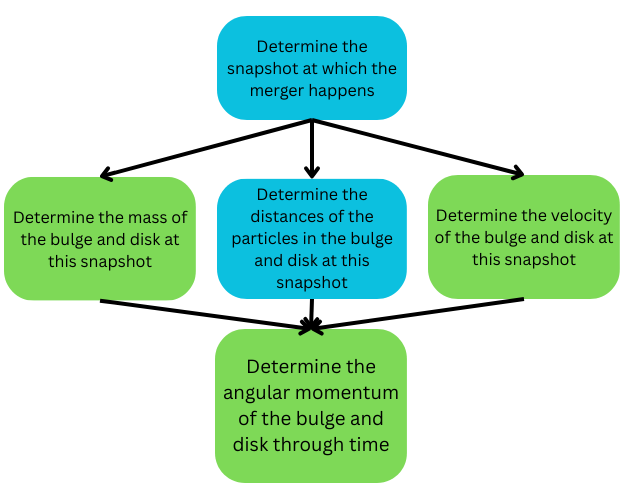
\includegraphics[width = 0.45\textwidth]{Updated Figure 2.png}
    \label{Figure 2}
    \caption{Flow Chart showing anticipated stages of this research. The green shows the data that will be plotted while the blue shows the data that will be used within the plots, but not explicitly plotted itself.}
\end{figure}


%What is my hypothesis for what I will find, and why do I think this will occur?
Based on the preceding information, my hypothesis is that we will find a merger remnant that has an elliptical shape. This implies that there will be relatively low angular momentum as well as a more uniform density distribution than before the merger. Furthermore, since it will likely result in an elliptical galaxy, there will not be a component that is noticeably rotating. I further anticipate the velocity dispersion to be somewhat even and somewhat low as elliptical galaxies do not show significant rotation as compared to spiral galaxies. I believe this is the likely scenario considering previous work done that shows a merger is imminent, and information from these papers and from what we have learned and done in classes to explain galactic mergers. 

%\software{astropy \citep{2013A&A...558A..33A,2018AJ....156..123A},  
          %Cloudy \citep{2013RMxAA..49..137F}, 
          %Source Extractor \citep{1996A&AS..117..393B}
          %}

%\section{Bibliography}
%\bibliography{Research Project}{}
\bibliography{bibliography}


\end{document}